\documentclass[twoside, 11pt]{article}

\usepackage[sc]{mathpazo} % Use the Palatino font
\usepackage{textcomp}
\usepackage[T1]{fontenc} % Use 8-bit encoding that has 256 glyphs
\linespread{1.05} % Line spacing - Palatino needs more space between lines
\usepackage{microtype} % Slightly tweak font spacing for aesthetics

\usepackage[english]{babel} % Language hyphenation and typographical rules

\usepackage[hmarginratio=1:1,top=32mm,columnsep=20pt]{geometry} % Document margins
\usepackage[hang, small,labelfont=bf,up,textfont=it,up]{caption} % Custom captions under/above floats in tables or figures
\usepackage{booktabs} % Horizontal rules in tables

\usepackage{lettrine} % The lettrine is the first enlarged letter at the beginning of the text

\usepackage{enumitem} % Customized lists
\setlist[itemize]{noitemsep} % Make itemize lists more compact

\usepackage{abstract} % Allows abstract customization
\renewcommand{\abstractnamefont}{\normalfont\bfseries} % Set the "Abstract" text to bold
\renewcommand{\abstracttextfont}{\normalfont\small\itshape} % Set the abstract itself to small italic text

\usepackage{titlesec} % Allows customization of titles
\renewcommand\thesection{\Roman{section}} % Roman numerals for the sections
\renewcommand\thesubsection{\arabic{subsection}} % roman numerals for subsections
\titleformat{\section}[block]{\large\scshape\centering}{\thesection.}{1em}{} % Change the look of the section titles
\titleformat{\subsection}[block]{\large}{\thesubsection.}{1em}{} % Change the look of the section titles

\usepackage{fancyhdr} % Headers and footers
\pagestyle{fancy} % All pages have headers and footers
\fancyhead{} % Blank out the default header
\fancyfoot{} % Blank out the default footer
\fancyhead[C]{F70 - Mechanik und Vakuum $\bullet$ April 2018 $\bullet$ Thimo Preis \& Tobias Abele} % Custom header text
\fancyfoot[RO,LE]{\thepage} % Custom footer text

\usepackage{titling} % Customizing the title section

\usepackage{hyperref} % For hyperlinks in the PDF
\hypersetup{bookmarks=true,bookmarksopen=true}

%----------------------------------------------------------------------------------------
%\usepackage[backend=biber,
%style=numeric,
%bibencoding=ascii
%]{biblatex}
%\addbibresource{Bibliography.bib}
%	TITLE SECTION
%----------------------------------------------------------------------------------------

\setlength{\droptitle}{-4\baselineskip} % Move the title up

\pretitle{\begin{center}\Huge\bfseries} % Article title formatting
	\posttitle{\end{center}} % Article title closing formatting
\title{F70: Mechanik und Vakuum} % Article title
\author{%
	\textsc{Thimo Preis and Tobias Abele}\thanks{Betreut von ...} \\[1ex] % Your name
	\normalsize Ruprecht-Karls-Universität Heidelberg
	%\normalsize 
}
\date{16.04-20.04.2018}


\usepackage{physics}
\usepackage{amsmath}
\usepackage{amssymb}
\usepackage{wasysym}
\usepackage{floatflt}

\usepackage{graphicx}
\usepackage{tikz}
\usetikzlibrary{shapes,calc,intersections,arrows.meta}
\usetikzlibrary{patterns,circuits.ee.IEC}
\usepackage{pgfplots}
\pgfplotsset{compat=1.15}

	

\begin{document}
	

	\maketitle
	
		\begin{abstract}
		\noindent
	\label{Abstract}
\noindent
The goal of this experiment is to do research on the characteristics of the muon. In detail we want to determine the lifetime and polarization of cosmic muons, which would also prove parity-violation in the weak interaction. For all our measurements we have six layers of scintillators with metal in between. Furthermore we can add a homogeneous magnetic field so that the muon will do a larmor-precession around the direction of the field. This makes it possible to determine the larmor-frequency, the magnetic moment of the muon and the polarization. The evaluation was done with ROOT.

\begin{table}[h]
	\centering
\begin{tabular}{lll}
	\toprule
	Physical Property & Abbreviation & Measured Value \\
	\midrule
	Lifetime & $\tau _{0}$ & $\left(2229 \pm 40.6_{stat} \pm 24.36_{sys} \right)\mathrm{ns}$\\
	
	Capture Lifetime & $\tau _{C}$ & $\left(961.1 \pm 110.8_{stat} \pm 79.11_{sys} \right) \mathrm{ns}$\\
	
	Coupling Constant& $G_F$&$\left(1.155 \pm 0.035 \right)\times 10^{-11} \mathrm{MeV} ^{-2}$\\
	
	Larmor Frequency & $\omega _{Larmor}$ &$\left(3.342 \pm 0.028_{stat} \pm 0.041_{sys}\right) \mathrm{MHz}$\\
	
	Magnetic Moment & $\mu _{mu}$ & $\left(2.75 \pm 0.04\right)\times 10^{-7} \mathrm{eV T^{-1}}$\\
	
	Polarization & P & $\left(0.23 \pm 0.11_{stat} \pm 0.03_{sys}\right)$\\
	\bottomrule
\end{tabular}
\caption{Measured Values}
\label{tab:1.Tab}
\end{table}
\end{abstract}
	\section{Theory}
\subsection{Relaxation time}
A macroscopic probe consists of many atoms, each of which with a nucleus carrying a spin and thus a magnetic dipole moment $\mu _I = \hbar \gamma _I \vec{I}$. The spins try to align either in a parallel or an antiparallel way with respect to an external magnetic field $B_0$. Restricting the discussion to protons we expect an effective magnetization in direction of $\vec{B}_0$ due to them having the tendency to occupy the energetically more favorable state, according to the Fermi-Dirac statistic. Disrupting the macroscopic magnetization from equilibrium will always lead to the same macroscopic magnetization after some time, because the system wants to minimize its total energy according to the principle of least action. This process is called relaxation and we distinguish between two different kinds of relaxation.\cite{manual} \cite{MRI}

\subsubsection{Spin-Spin relaxation $T_2$}
The spin-spin relaxation is caused by the interaction between distinct spins amongst themselves. The transverse magnetization gets decreased via the dephasing of the coherent movement of the spin magnetic moments. The characteristic relaxation time of this process is called spin-spin relaxation time $T_2$.
The Bloch equations describe the time evolution of the magnetization subject to relaxation. From them one can derive the time evolution of the transverse magnetization to be determined by the spin-spin relaxation time via \cite{manual}
\begin{equation}
	M_{\perp} (t) = M^0 _{\perp}\, e^{-\frac{t}{T_2}}\mathrm{.}
	\label{eq:1}
\end{equation}
\subsubsection{Spin-Lattice relaxation time $T_1$}
 The spin-lattice relaxation time describes the interaction between the spins with the external magnetic field. The energy emitted by a system out of equilibrium dissipating to its equilibrium state, thus attaining an effective equilibrium magnetization, is absorbed by the lattice. The characteristic time scale of this relaxation process caused in this interaction is called spin-lattice relaxation time $T_1$. The time evolution of the magnetization component (anti-)parallel to the external magnetic field $B_0$ is again determined by the Bloch equations via the spin-lattice relaxation time to be \cite{manual} \cite{MRI}
 \begin{equation}
 	M_{\parallel}(t) = M^0 _{\parallel} \, \left(1-2\, e^{-\frac{t}{T_1}}\right)\mathrm{.}
 	\label{eq:2}
 \end{equation}

\subsection{Chemical shift}
Chemical shift is, besides dipole-dipole interaction and internal coupling, one of the main internal interactions of magnetic dipole moments. It accounts for an additional magnetic field caused by the electrons surrounding the magnetic dipole moments of the nucleus. The factor of proportionality between the additional and the external magnetic field is molecule specific and is called magnetic shielding factor (measured in parts per million). The Hamiltonian of the observed system is given by 
\begin{equation}
	H = H_Z + H_C + H_J + H_D\mathrm{,}
	\label{eq:3}
\end{equation}  
where $H_Z$ represents the Zeeman splitting caused by the external magnetic field $B_0$ and $H_D$ accounts for the dipole-dipole interaction (is averaged out in fluids). The electrons weaken the magnetic field around the nucleus proportionally to the external magnetic field, following Lenz´s law, which in turn results in the chemical shift $H_C = \hbar \gamma \sigma \vec{I}\vec{B}_0$. The additional term $H_J = J_{12} \vec{I}_1 \vec{I}_2$ is caused by the indirect coupling between two magnetic dipole moments in a molecule via the electrons, $J_{12} $ describes the coupling factor.
The Brownian motion is responsible for averaging out the splitting of the spectrum caused by the indirect coupling in different molecules.\cite{Hornak} \cite{IndirectCoupling}

\subsection{Imaging with NMR}
\label{sec:3}
A static, spatially homogeneous magnetic field is not sufficient for image taking, because all spins would have the same Larmor frequency. One excitation pulse would therefore always excite the entire sample. We can spatially localize the amount of hydrogen atoms at one point by applying a gradient field, because the Larmor frequency is proportional to the magnetic field, which in turn is proportional to the spatial position.
We can split the sample into slices in e.g. the xy-plane by applying a magnetic gradient in z-direction, because this results in the precession motion of every slice to have a different Larmor frequency:
\begin{equation}
	\omega _{Larmor} = \gamma \left(B_0+ B^z (z)\right)\mathrm{.}
	\label{eq:4}
\end{equation}
One can therefore guarantee spins of a specific slice to go in resonance with the frequency applied to the rotating magnetic field and then measure the relaxation time, this is called frequency coding. The stronger the applied magnetic gradient the thinner a given slice in the xy-plane becomes.\\
We can furthermore apply a phase encoding gradient to dephase spins along the vertical axis (y-axis). The gradient is only applied for a short amount of time such that, after the gradient has been shut down, we observe several phases between the spins along the y-axis, hence we now can decode the y-position via the phase with a spin echo measurement (compare section \ref{sec:1}), this is called phase coding. The resolution of this localization is limited by the measurement only being able to distinguish two phases with a difference less than $2 \pi$.\\
We can finally apply a third gradient field in x-direction during the echo, this results in the z-gradient field to increase along the x-direction such that the Larmor frequencies along the x-axis increase with an increase in magnetic field strength. The measured echo of the magnetic resonance signal now consists of a broad frequency spectrum, but now we can identify the spatial point via the specific Larmor frequency. One can then use either frequency or phase coding in order to acquire a 1D image of the sample via a 1D Fourier transformation of the measured NMR signal, where every point in position space corresponds either to a specific frequency or a specific phase.\\
One can also use both methods in order to make a 2D image measurement. One first selects a slice by an appropriate combination of gradient field and high frequency pulse. Within the slice, 2D position information is derived by a combination of phase coding in x-direction and frequency coding in y-direction. One then proceeds to make N measurements, each consisting of a combination of frequency and phase coding, with different values of the phase coding gradients in x-direction. During every measurement the NMR signal is read out at different times $t_m$ with $m \in \{1,M\}$. The $2\times2$ D matrix of the image is then finally derived via a two dimensional Fourier transformation of the matrix consisting of $N\times M$ data points.\cite{manual} \cite{ernst1987principles}
	\section{Experimental setup and measurement principles}
\subsection{Measurement of relaxation times and chemical shift}
In the first part of the experiment the spin-lattice relaxation time $T_1$ and the spin-spin relaxation time $T_2$ are measured. The spin-spin relaxation time is measured by the spin echo (compare section \ref{sec:1}) as well as by the Carr-Purcell method (compare section \ref{sec:2}). The chemical shift of protons is measured in the following and used to identify five different substances. These measurements are carried out with a Bruker minispec p20, it consists of a Minispec p20 Electronic Unit used signal generation and of a Minispec p20 magnet with a static magnetic field $B_0$. The magnet is shielded by Styrofoam for minimal termperature variation when in use. One can now generate a magnetization $M_{\perp}$ perpendicular or  $M_{\parallel}$ antiparallel to $\vec{B}$ by applying a high frequency pulse $\omega_{HF}$ via the electronic unit to the ground state magnetization $\vec{M}$. We can now rotate the macroscopic magnetization by an angle $\alpha = \gamma_I B_1 \Delta t$ by applying a sinusoidal voltage of given frequency $\omega _{HF}$ for a given time duration $\Delta t$ to a coil oriented perpendicular to the static magnetic field $B_0$. This results in a solenoidal magnetic field $\vec{B}_1$ which is longitudinally polarized in a parallel way with respect to the orientation of the coil. The rotated macroscopic magnetization now precesses around the $B_0$ magnetic field. This in turn induces a voltage into the same coil, which then again represents our measurement signal, which is a mixed signal partially consisting of the so-called working frequency. It is the difference $\nu_{work}=\omega_{HF} - \omega_{Larmor}$ and it has to be calibrated to a value of around $1 kHz$ by varying the Larmor frequency via varying the static magnetic field. The optimal Larmor frequency can be calculated with $\omega_{HF} = 19.8 \mathrm{MHz}$ to be $\omega_{Larmor} = 19.799 \mathrm{MHz}$. The working frequency varied during the measurement by $\pm 50 \mathrm{Hz}$ due to variations in the magnetic field. With $\omega_{Larmor} = \gamma B_0$ we can therefore assume the magnetic field to vary by $\Delta B_0 \approx 5.2\times10^{-5} T$ whilst the temperature of the apparatus changed by $\Delta T \approx 0.01$ \textcelsius. Thus, the systematic error in the calibrated working frequency due to temperature variations can be estimated to be around $\Delta \nu_{work,sys} = 5 \% \nu_{work}$.\\
One can vary the time duration of the applied voltage in order to rotate the magnetization by an angle $\alpha = 90$ \textdegree, 180 \textdegree \, into its perpendicular or antiparallel component with respect to the orientation of $\vec{B} _0$.\cite{manual}


\subsubsection{Spin echo} 
\label{sec:1} In order to measure the spin-spin relaxation time $T_2$ according to equation \ref{eq:2} one starts with a 90 \textdegree\, pulse in order to create a transverse magnetization in y-direction, such that it will precess around the static magnetic field $B_0$ with a given Larmor frequency $\omega_{Larmor} = \gamma B_0$.
\begin{figure}[h]
	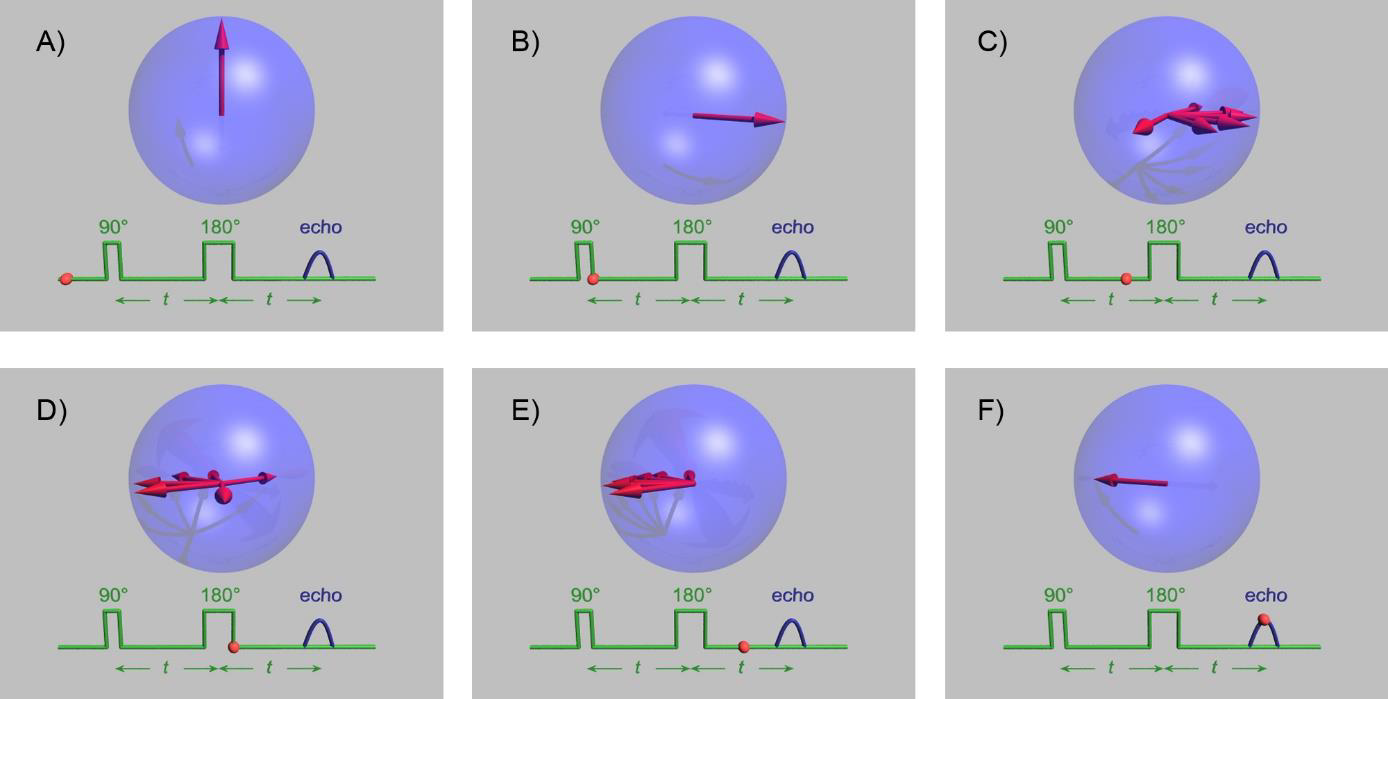
\includegraphics[width=75mm
	]{Spinecho}
	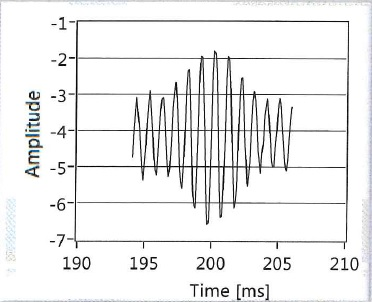
\includegraphics[width=75mm]{Spinecho2}
	\centering
	\caption{\itshape From left to right: Spin echo method \cite{Spinecho}, output signal \cite{manual}}
	\label{fig:1}
\end{figure}
\newpage
\noindent
 Protons at different positions in the probe will now precess with different Larmor frequencies due to the non-linearity of the field, thus phase difference between the protons will develop.
One can now revert the phases of the spins with a 180\textdegree\, pulse in order to guarantee all protons of given phases to coherently align after a given time interval of two times the so-called spin-echo time $\tau$. The induced signal then again represents the relaxation time for the transverse magnetization, which is dominantly caused by spin-spin interactions, thus $T_2$. \cite{manual} \cite{MRI}

 

\subsubsection{Carr-Purcell sequence}
\label{sec:2}
One only achieves approximate alignment of the magnetic dipole moments after $2 \tau$ for long spin echo times due to molecular diffusion happening before the 180 \textdegree\, pulse can be applied. The Carr-Purcell sequence minimizes the effects of molecular diffusion and field inhomogeneities by starting the sequence with a 90 \textdegree\, pulse followed up by a 180 \textdegree\, pulse to ensure phase coherence of the system after $t=2\tau$. One now applies further 180 \textdegree\, pulses for every odd multiple of $\tau$ in order to guarantee phase coherence for every even multiple of $\tau$.
\begin{figure}[h]
	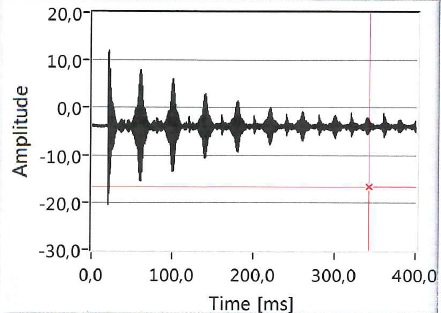
\includegraphics[width=120mm]{CarrPurcell}
	\centering
	\caption{\itshape Carr-Purcell sequence \cite{manual}}
	\label{fig:2}
\end{figure} 
\noindent
A measurement of the spin-spin relaxation time by the Carr-Purcell method hence yields a value which is closer to the true value of the system as compared to the measurement with the spin echo method.\cite{manual}
\label{sec:5}

\subsubsection{Measurement of spin-lattice relaxation $T_1$}

One produces a magnetization antiparallel to the static magnetic field by starting the measurement with the generation of a 180 \textdegree\, pulse. By following this up with a 90 \textdegree\, pulse one measures a signal which represents the current longitudinal magnetization, which is due to spin-lattice interactions and can therefore be used to measure $T_1$.\cite{manual}
\begin{figure}[h]
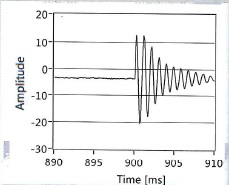
\includegraphics[width=100mm]{T_1}
\centering
\caption{\itshape Pulse sequence 180 \textdegree-90 \textdegree with $\tau$ = 20ms \cite{manual}}
\label{fig:3}
\end{figure}
\subsection{Imaging with NMR}
The imaging measurements are made with the Bruker NMR analyzer mq7.5, where the gradient fields where applied via a system of Helmholtz coils. Nuclear Magnetic Resonance techniques are used for imaging measurements in one and two dimensions. The flow of oil in sand is measured as a time dependent process in one dimension. Two dimensional measurements are carried out to map the inner volume of substances which contain oil or water. The measurement principle of this apparatus is described within section \ref{sec:3}.\cite{manual}

	\section{Auswertung}
\subsection{Drehschieberpumpe}
%Hier 2.1 Beobachtungen, Fragen
%Prinzip einer Drehschieberpumpe



\subsection{Abpumpen kondensierbarer Dämpfe}
%Hier 2.2 Beobachtungen, Fragen,Auswirkung Gasballast
\begin{figure}[h]
	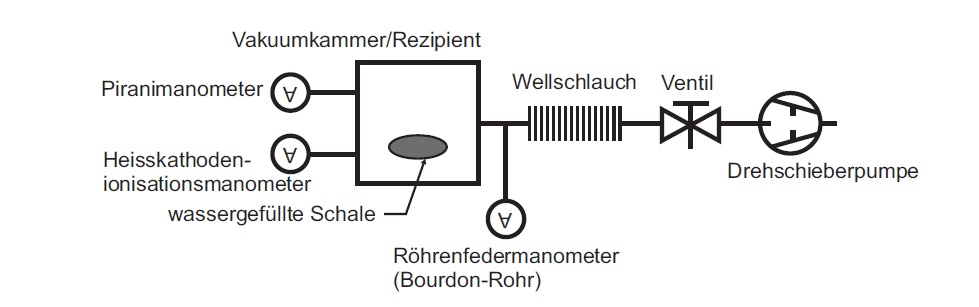
\includegraphics[width=100mm]{Dampf}
	\centering
	\caption{\itshape Blockschaltbild zum Abpumpen kondensierbarer Dämpfe}
	\label{fig:1}
\end{figure}
\noindent

\subsection{Molekular-und Turbomolekularpumpe}
%Hier 2.3, Funktionsweise TMP, mit Gaedestufe, siehe TMP Herstellerangaben hier, kannst einfach die in Anleitung gefragten Werte sonst abschreiben
\begin{figure}[h]
	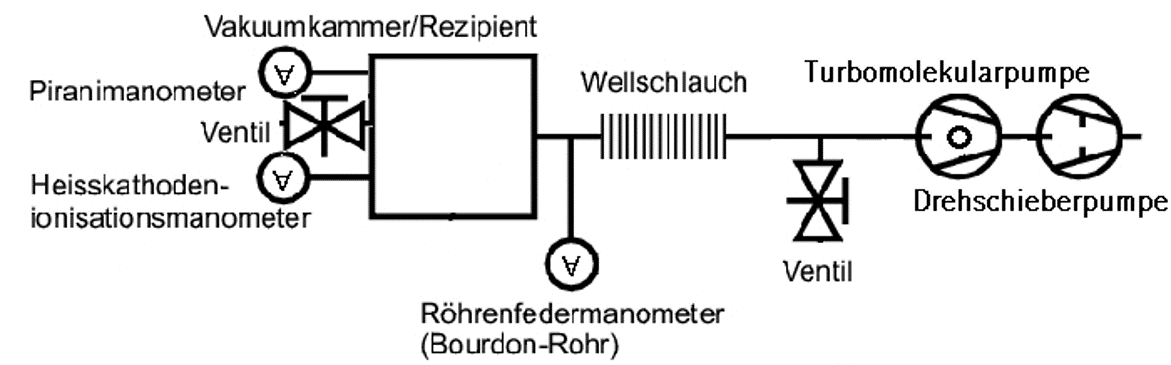
\includegraphics[width=100mm]{TMPmitVorpumpe}
	\centering
	\caption{\itshape Blockschaltbild der Turbomolekularpumpe mit Drehschieberpumpe als Vorpumpe}
	\label{fig:2}
\end{figure}
\noindent

\subsection{Saugvermögen der TMP}
%Hier 2.4, 

\begin{figure}[h]
	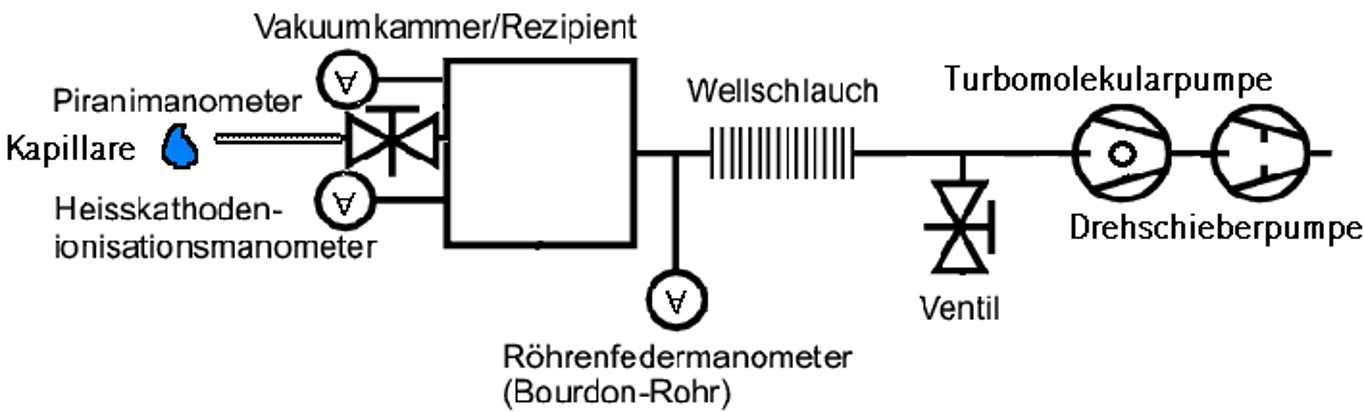
\includegraphics[width=100mm]{Saug}
	\centering
	\caption{\itshape Blockschaltbild Saugvermögen der TMP}
	\label{fig:3}
\end{figure}
\noindent


%\begin{figure}[h]
%	\includegraphics[width=100mm]{SaugvermögenDruck}
%	\centering
%	\caption{\itshape Saugvermögen als Funktion des Logarithmus des Drucks}
%	\label{fig:4}
%\end{figure}
\noindent
\newpage
\subsection{Leitwert von Rohr und Blende}
%Hier 2.5

\begin{figure}[h]
	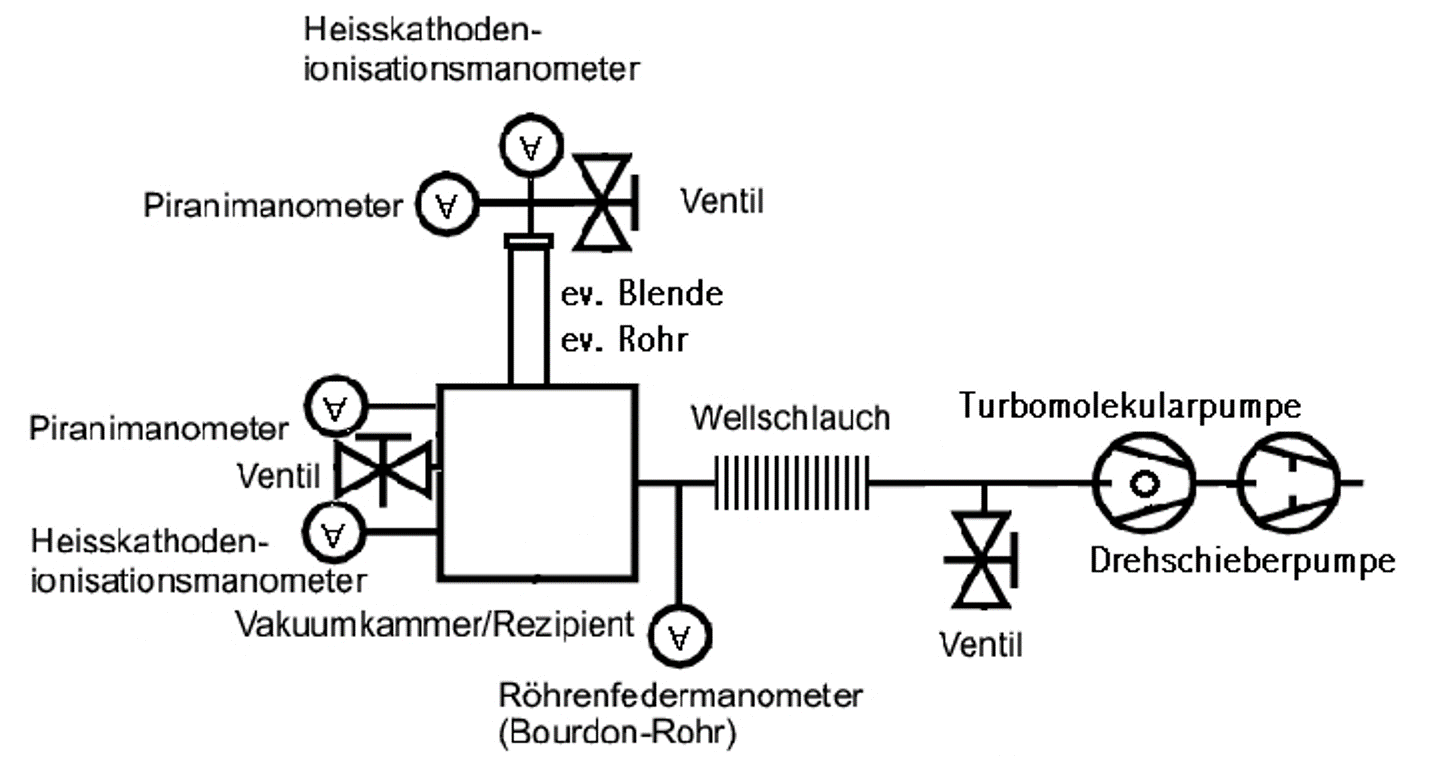
\includegraphics[width=100mm]{LeitwertVonRohrUndBlende}
	\centering
	\caption{\itshape Blockschaltbild Saugvermögen der TMP}
	\label{fig:5}
\end{figure}

%\begin{figure}[h]
%	\includegraphics[width=100mm]{Leitwer1}
%	\centering
%	\caption{\itshape Leitwert von als Funktion des Logarithmus des Drucks}
%	\label{fig:6}
%\end{figure}
\noindent


%\begin{figure}[h]
%	\includegraphics[width=100mm]{Leitwert2}
%	\centering
%	\caption{\itshape Leitwert von als Funktion des Logarithmus des Drucks}
%	\label{fig:7}
%\end{figure}
\noindent



\subsection{Lecksuche}
%Hier 2.6

\begin{figure}[h]
	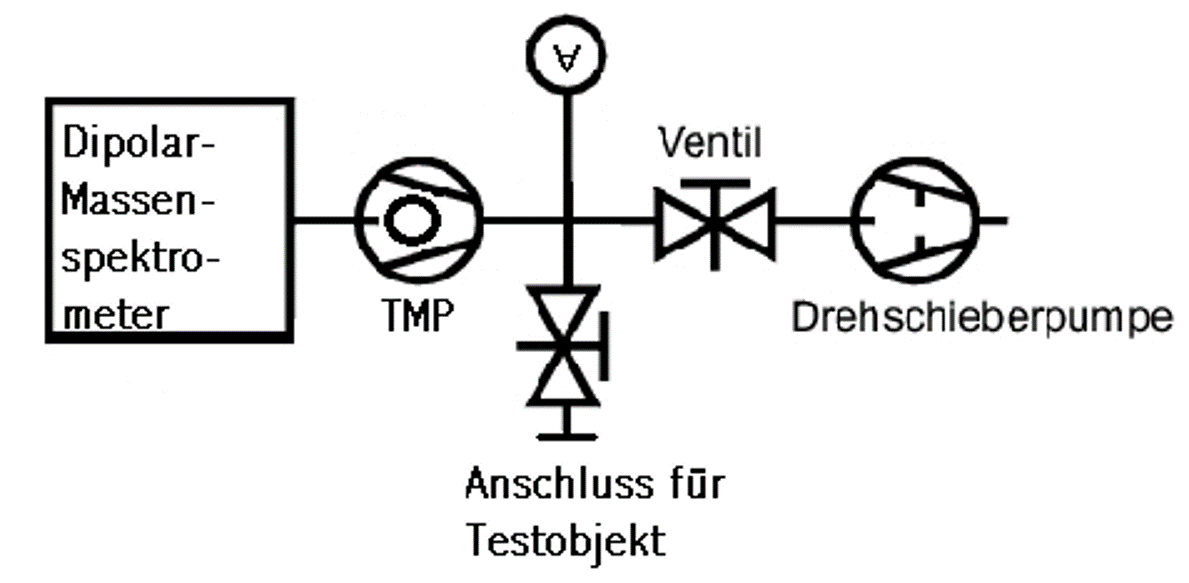
\includegraphics[width=100mm]{GegenstromLecksuche}
	\centering
	\caption{\itshape Blockschaltbild Lecksuche}
	\label{fig:8}
\end{figure}

	
\section{Discussion - Thimo Preis}
The setup in the first two parts of the experiment was not isolated very well thermally such that the $B_0$ magnetic field was very sensitive to work with. The skew available for varying $B_0$ is furthermore very unprecise and does not increase or decrease $B_0$ consistently with a consistent rotating motion. It was therefore very difficult to calibrate the working frequency, which again is only necessary due to the ineffective thermal shielding with styrofoam, consistently after every measurement due to the unprecise adjustability of $B_0$. One should therefore improve the thermal shielding of the Minispec p20 magnet in order to render the ongoing calibration of the working frequency after every measurement unnecessary in the boundaries of the setups precision. One should furthermore increase the number of possible data points for the used fit of $T_1$ and $T_2$ in order to increase the precision of the measured values. This can easily be achieved by expanding the available LabView program to guarantee more than ten data points to be accounted for in the fit. One could furthermore refine the step size of the switches of the Minispec p20 electronic unit in order to account for more data points in the steeply falling/rising range of the exponential decay/rise. In total it would improve the precision of the measured results, if one would simply increase the number of taken data points during the measurement and also increase the number of measurements and thus improve on the fits in order to average out the huge systematic errors due to the sensitivity of the apparatus on the chosen peak window and on the thermal shielding.  One should furthermore be provided with theoretical values of the relaxation times in order to guarantee a successfull discussion of the measured values and a prompt error evaluation during the experiment for measured values way off the theoretical values. These error sources had a higher impact on the first part of the measurement than on the second part concerned with the chemical shift. The systematic errors averaged out due to the structure of the measurement relying only on differences between the peaks.\\
\\
The third part of the experiment went very smooth as the Bruker NMR analyzer mq7.5 was thermally shielded very well (compare \ref{sec:4}) and had a high image resolution, only the intrinsic magnetic field non-linearities distorted our images a bit. By trying out the different slicing methods we could nevertheless 
achieve images of high resolution from which we could draw important physical conclusions.\\
The instruction manual \cite{manual} gives a clear introduction to the NMR concepts. The third part concerned with "Imaging with NMR" is to in depth for this experiment and misses to convey the quintessential points of this method. One should therefore cut down the explanation of the actual Fourier transformation of the NMR signal and in contrast should go more in depth in explaining the actual two dimensional data aquisition and on how the Helmholtz coils were set up in order to guaruantee linear gradient fields.
\\
Altogether this experiment is very instructive in conveying the import NMR methods used throughout the medical and food sector in an engaging way. Only the first part of the experiment could be improved in order to increase the precision of the measured results as discussed above.
	\section{Diskussion}

	\begin{thebibliography}{9}
		\bibitem{manual} 
		F61 - Nuclear Magnetic Resonance in the Advanced Students Laboratory. Url: \\\texttt{https://www.physi.uni-heidelberg.de/Einrichtungen/FP/anleitungen/F61.pdf}
	
		\bibitem{Gadolinium}
		Gadolinium Wikipedia article, Last Access: 02/04/2018 20:24, Url: \\
		\texttt{https://en.wikipedia.org/wiki/Gadolinium}
		
			
		\bibitem{Hornak} 
		The Basics of NMR by Joseph P. Hornak
		URL: \\\texttt{http://www..cis.rit.edu/htbooks/nmr}
		
		
		\bibitem{IndirectCoupling}
		Indirect dipole-dipole coupling, Last Access: 02/04/2018 20:24, Url: \\
		\texttt{https://en.wikipedia.org/wiki/J-coupling}
		
		\bibitem{diffusion}
		„Diffusions-Poren-Bildgebung mittels kernmagnetischer Resonanz"
		Dissertation of Tristan Anselm Kuder, University Heidelberg(2014)\\
		
		\bibitem{Spinecho}
		Spin echo method, Last Access: 02/04/2018 20:24, Url: \\
		\texttt{https://en.wikipedia.org/wiki/Spin\_echo}
		
		\bibitem{MRI}
		Wie funktioniert MRI? By Weishaupt, Dominik in Springer 2014, ISBN: 978-364-24161-6-3

		\bibitem{Fluorine}
		Fluorine atom information, Last Access: 02/04/2018 20:24,Url: \\
		\texttt{https://en.wikipedia.org/wiki/Fluorine}
		
		\bibitem{ernst1987principles}
		Principles of nuclear magnetic resonance in one and two dimensions by 
		Ernst, Richard R and Bodenhausen, Geoffrey and Wokaun, Alexander and others. Volume 14, 1987, Clarendon Press Oxford.
		
	\end{thebibliography}
	
\end{document}